% !TeX program = lualatex
%======================================================================
% DOCUMENT SETUP -- compile with recent LuaLaTeX
%======================================================================
% Metadata must appear before \documentclass.
\DocumentMetadata{
  tagging=on,
  tagging-setup={math/setup=mathml-SE},
  pdfstandard=ua-2,
  lang=en-US
}
\documentclass[10pt,letterpaper]{article}
\usepackage{notes}
% \usepackage[widemargin]{notes}

%----------------------------------------------------------------------
% PDF PROPERTIES -- title for this lecture; author/course from notes.sty
%----------------------------------------------------------------------
\hypersetup{
  pdflang={en-US},
  pdftitle={\class{} - 2.6 Method of Undetermined Coefficients - Part 2},
  pdfauthor={\instructor},
  pdfsubject={\coursename}
}

% Standalone lecture: compile this file from the repository root.
% Keep notes.sty on the TeX search path. The original 2.6-mouc.tex is unchanged.
% Timing comments describe a suggested 9:00--9:50 class; optional extensions
% remain in the notes for independent reading or a longer class.
\begin{document}
\lesson[Logan, Differential Equations, 3rd edition\enspace\textbullet\enspace Section 2.3.1]
  {2.6, Part 2}{Repairing the Trial}
\renewcommand{\lessontitle}{Undetermined Coefficients, Part 2}

% SIDE NOTE: 9:00 | Try the Method Again
% a) Recall x = x_h + x_p and the exponential trial.
% b) Present the equation as an ordinary exercise; do not announce the exception.
% c) Let students discover that every A gives zero.
\section{Trying the Method Again}
\subsection{A Familiar-Looking Problem}
Last time, we chose a trial based on the forcing term, substituted it into
the equation, and solved for its coefficients. Let's try the same steps again.

\begin{example}{Find the general solution to $x''-4x=e^{2t}$.}
We follow the same approach as last time. Consider
\[
x''-4x=e^{2t}.
\]
The homogeneous solution is
\[
x_h(t)=c_1e^{2t}+c_2e^{-2t}.
\]
\textbf{Try the familiar approach.} What trial would you choose?
Our initial guess would be $x_p(t)=Ae^{2t}$, but substituting
gives
\[
x_p''-4x_p=4Ae^{2t}-4Ae^{2t}=0.
\]
No choice of $A$ can make this equal to $e^{2t}$.
The trial function already solves the homogeneous equation.

\textbf{Pause and diagnose the failure.}
This is not an algebra mistake. Every multiple of $e^{2t}$ solves the
homogeneous equation, so changing $A$ will always leave zero on the left.
Adding $Be^{-2t}$ would not help either: that term also solves the homogeneous equation.
We need a function outside this homogeneous family.

\textbf{Try a new form.} Multiply the guess by $t$:
\[
x_p(t)=Ate^{2t}.
\]
Then
\[
x_p'=(A+2At)e^{2t},
\qquad
x_p''=(4A+4At)e^{2t}.
\]
Substituting into the nonhomogeneous equation gives
\[
x_p''-4x_p=4Ae^{2t}=e^{2t},
\]
so $A=\frac14$. Therefore,
\[
\boxed{x(t)=c_1e^{2t}+c_2e^{-2t}+\frac14te^{2t}.}
\]


\end{example}
\subsection{Why Did Multiplying by $t$ Help?}
The derivatives of $Ate^{2t}$ contain extra terms because of the product rule.
The terms involving $te^{2t}$ cancel, but the extra $4Ae^{2t}$ survives.
That remaining term has exactly the form needed to match the forcing.

Compare the two attempts:
\[
\begin{array}{c|c}
\text{Trial} & x_p''-4x_p\\\hline
Ae^{2t}&0\\
Ate^{2t}&4Ae^{2t}
\end{array}
\]
The DE has solutions; it was our first trial family that was too restrictive.

% SIDE NOTE: 9:10 | The Duplicate Rule
% a) Compare whole functions with x_h, including exponential factors.
% b) Multiply the overlapping trial group by t.
% c) Repeated roots may require t squared.
\section{The Duplicate Rule}
\subsection{Recognizing the Overlap}
\textbf{Duplication} occurs when a term in the trial family is already
part of the homogeneous solution. Such a term contributes zero when
substituted into the left-hand side.

The \textbf{duplicate rule} is: multiply the overlapping trial group by
$t^s$, where $s$ is the smallest nonnegative integer that removes the overlap
with the homogeneous solution. For a second-order equation, $s$ is $0$, $1$, or $2$.
Apply this correction \emph{before} differentiating the trial.

\subsection{When One Factor of $t$ Is Not Enough}
\begin{example}{Find the general solution to
\[
x''+2x'+x=e^{-t}.
\]}
\textbf{Step 1. Find the homogeneous solution.}
The characteristic equation is $(\lambda+1)^2=0$. Thus
\[
x_h=c_1e^{-t}+c_2te^{-t}.
\]
\textbf{Step 2. Choose and repair the trial.}
Our first trial $Ae^{-t}$ duplicates a homogeneous term. Multiplying by $t$
gives $Ate^{-t}$, which is still a duplicate. Therefore, try
\[
x_p=At^2e^{-t}.
\]
\textbf{Step 3. Determine the coefficient.}
The derivatives are
\[
x_p'=A(2t-t^2)e^{-t},\qquad
x_p''=A(2-4t+t^2)e^{-t}.
\]
Substitute and collect terms:
\begin{align*}
x_p''+2x_p'+x_p
 &=A\bigl[(2-4t+t^2)+2(2t-t^2)+t^2\bigr]e^{-t}\\
 &=2Ae^{-t}.
\end{align*}
Thus $2A=1$, and the general solution is
\[
\boxed{x=c_1e^{-t}+c_2te^{-t}+\frac12t^2e^{-t}.}
\]
\end{example}
The repeated \textbf{characteristic root} explains why two factors of $t$
were needed. Always compare with the complete homogeneous solution.

\subsection{Which Terms Should Be Multiplied?}
\begin{example}{Choose an appropriate trial for $x''+x=\cos t+7$.
Do not solve for its coefficients.}
The homogeneous solution is $x_h=c_1\cos t+c_2\sin t$.
The usual trial would be $A\cos t+B\sin t+C$.
The sine and cosine group overlaps with $x_h$, but the constant does not.
Therefore,
\[
\boxed{x_p=t(A\cos t+B\sin t)+C.}
\]
Multiply the \emph{entire sine/cosine group} by $t$, and leave the constant alone.
\end{example}

\subsection{Compare the Whole Function}
The functions $\cos t$ and $e^{-t}\cos t$ are different. If
$x_h=e^{-t}(c_1\cos t+c_2\sin t)$ and $f(t)=\cos t$, then
$A\cos t+B\sin t$ does not duplicate the homogeneous solution.
Likewise, $\cos t$ and $\cos 2t$ have different frequencies.

% SIDE NOTE: 9:22 | Choose, Check, Repair
% a) Have students give the trial before showing the solution.
% b) Ask which group overlaps and how many t factors are needed.
% c) Parts 4 and 5 are optional extensions if time is short.
\subsection{Practice the Complete Decision}
\begin{example}{Choose an appropriate trial for each equation. Do not solve for the coefficients.
\begin{enumerate}
\item $x''-4x=e^{-2t}+t$.
\item $x''+4x=3\sin 2t$.
\item $x''+2x'+2x=\cos t$.
\item $x''-3x'+2x=te^t$.
\item $x''=t^2+1$.
\end{enumerate}}
\begin{enumerate}
\item The roots are $\pm2$. Repair only the exponential group:
\[x_p=Ate^{-2t}+Bt+C.\]
\item The homogeneous family contains both waves of frequency $2$:
\[x_p=t(A\cos 2t+B\sin 2t).\]
\item The homogeneous family is $e^{-t}(c_1\cos t+c_2\sin t)$.
There is no overlap with the trial
\[x_p=A\cos t+B\sin t.\]
\item The roots are $1$ and $2$. Start with $(At+B)e^t$ and
multiply the whole polynomial/exponential group by $t$:
\[x_p=t(At+B)e^t.\]
\item Here $x_h=c_1+c_2t$. The initial quadratic trial overlaps with both
homogeneous terms. Multiplying it only by $t$ would still leave a linear term.
Use
\[x_p=t^2(At^2+Bt+C).\]
This is a repeated-root case with characteristic root $0$.
\end{enumerate}
\end{example}

\subsection{A Checklist for Any Problem}
\begin{enumerate}
\item Find $x_h$ from the characteristic equation.
\item Choose the initial trial from the forcing term, using sums and products.
\item Check for duplication and repair each overlapping group.
\item Substitute into the DE and determine the coefficients.
\item Write $x=x_h+x_p$.
\item Apply any initial conditions to this complete solution.
\end{enumerate}

% TRANSITION (blue box): We can now solve an IVP and interpret its motion.
% SIDE NOTE: 9:29 | A Forced Spring
% a) Translate displacement and release from rest into initial conditions.
% b) Find the particular solution, then apply the IC to the full solution.
% c) Distinguish the forced response from the decaying homogeneous part.
\section{Forced Springs and Long-Term Behavior}

\subsection{Forced Spring Model}

If an external force $F(t)$ acts on a spring-mass system,
Newton's second law gives
\[
mx''=-kx-\gamma x'+F(t),
\]
or
\[
\boxed{mx''+\gamma x'+kx=F(t).}
\]
This is a nonhomogeneous equation. We can use the method
of undetermined coefficients when $F(t)$ has a suitable form.

%-------------------------------------------------------------
\begin{example}{
A mass of $1$ kg is attached to a spring with spring constant
$2$ N/m and damping coefficient $2$ N\,s/m. An external
force $F(t)=4t$ N acts on the mass. Initially, the mass is
displaced $1$ m from equilibrium and released from rest.

Find the displacement $x(t)$.
}
The model and initial conditions are
\[
\begin{dcases}
x''+2x'+2x=4t,\\
x(0)=1,\\
x'(0)=0.
\end{dcases}
\]

First, solve the homogeneous equation. The characteristic
equation is
\[
\lambda^2+2\lambda+2=0
\implies \lambda=-1\pm i.
\]
Thus, the system is underdamped, with homogeneous solution
\[
x_h(t)=e^{-t}(c_1\cos t+c_2\sin t).
\]

For the linear forcing term, try
\[
x_p(t)=At+B.
\]
Then $x_p'=A$ and $x_p''=0$. Substituting gives
\[
2A+2(At+B)=4t.
\]
Matching coefficients yields
\[
2A=4,\qquad 2A+2B=0,
\]
so $A=2$ and $B=-2$. The general solution is
\[
x(t)=e^{-t}(c_1\cos t+c_2\sin t)+2t-2.
\]

Apply the initial conditions to the complete solution:
\[
x(0)=c_1-2=1
\implies c_1=3.
\]
Differentiating gives
\[
x'(t)=e^{-t}
\bigl[(c_2-c_1)\cos t-(c_1+c_2)\sin t\bigr]+2.
\]
Therefore,
\[
x'(0)=c_2-c_1+2=0
\implies c_2=1.
\]
The solution is
\[
\boxed{x(t)=e^{-t}(3\cos t+\sin t)+2t-2.}
\]
\end{example}

%-------------------------------------------------------------
% SIDE NOTE: 9:42 | Read the Two Pieces
% a) The homogeneous contribution decays in this damped example.
% b) Steady-state does not mean constant: the force is increasing.
% c) Different initial conditions change the transient.
\subsection{Transient and Steady-State Response}

The solution in the spring example has two parts:
\[
x(t)=
\underbrace{e^{-t}(3\cos t+\sin t)}_{\text{transient response}}
+
\underbrace{2t-2}_{\text{steady-state response}}.
\]
The homogeneous part is an oscillation with a decaying
amplitude. Since $x_h$ is short-lived
\[
x_h(t)\to0
\qquad\text{as }t\to\infty,
\]
we call it the \textbf{transient response}. Its coefficients
depend on the initial conditions, but its contribution
eventually becomes negligible.

The remaining part,
\[
x_p(t)=2t-2,
\]
is the \textbf{steady-state response}. It describes the
long-term motion driven by the external force. In particular,
\[
x(t)-(2t-2)\to0
\qquad\text{as }t\to\infty,
\]
so the graph of $x(t)$ approaches the line $x=2t-2$.
\begin{figure}[H]
\centering
%-------------------- Homogeneous solution --------------------
\begin{minipage}[t]{0.48\linewidth}
\centering
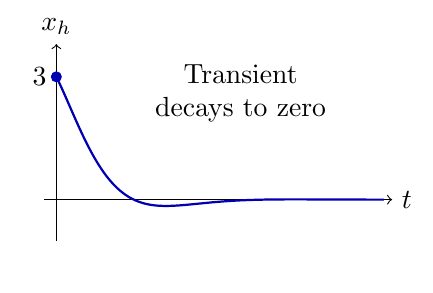
\begin{tikzpicture}[x=0.52cm,y=0.52cm]
    \path[use as bounding box] (-0.7,-1.6) rectangle (8.5,4.2);

    \draw[->] (-0.3,0) -- (8.2,0) node[right] {$t$};
    \draw[->] (0,-1) -- (0,3.8) node[above] {$x_h$};

    \draw[blue!70!black,thick,domain=0:8,samples=250]
        plot (\x,{exp(-\x)*(3*cos(deg(\x))+sin(deg(\x)))});

    \fill[blue!70!black] (0,3) circle (2pt);
    \node[left] at (0,3) {$3$};

    \node[align=center] at (4.5,2.6)
        {Transient\\decays to zero};
\end{tikzpicture}

\small (a) $x_h(t)=e^{-t}(3\cos t+\sin t)$
\end{minipage}
\hfill
%-------------------- Full solution --------------------
\begin{minipage}[t]{0.48\linewidth}
\centering
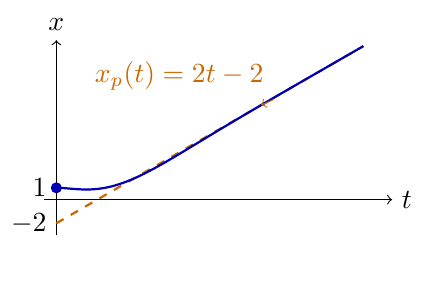
\begin{tikzpicture}[x=0.52cm,y=0.15cm]
    \path[use as bounding box] (-0.7,-5.55) rectangle (8.5,14.56);

    \draw[->] (-0.3,0) -- (8.2,0) node[right] {$t$};
    \draw[->] (0,-3) -- (0,13.5) node[above] {$x$};

    % Steady-state response
    \draw[orange!80!black,dashed,thick,domain=0:7.5]
        plot (\x,{2*\x-2});

    % Full solution
    \draw[blue!70!black,thick,domain=0:7.5,samples=250]
        plot (\x,{
            exp(-\x)*(3*cos(deg(\x))+sin(deg(\x)))
            +2*\x-2
        });

    \fill[blue!70!black] (0,1) circle (2pt);
    \node[left] at (0,1) {$1$};
    \node[left] at (0,-2) {$-2$};

    \node[orange!80!black,align=center] (steady) at (3,10.5)
        {$x_p(t)=2t-2$};
    \draw[->,orange!80!black] (steady.south east) -- (5,8);
\end{tikzpicture}

\small (b) $x(t)=x_h(t)+x_p(t)$
\end{minipage}
\caption{The transient decays, leaving the steady-state
response to describe the long-term motion.
The panels use different vertical scales.}
\end{figure}

Here, ``steady-state'' does not mean constant. The force
continues to increase, so the long-term displacement
increases as well. Next time, we will study periodic forcing. We will see how
the forcing frequency, the spring's natural frequency,
and damping affect the response, including the phenomena
of \textbf{beats} and \textbf{resonance}.



\subsection{What Changes with the Initial Conditions?}
Keep the same spring and force, but change the starting displacement or
velocity. The particular solution $2t-2$ still works. Only $c_1,c_2$ change:
\[
x=e^{-t}(c_1\cos t+c_2\sin t)+2t-2.
\]
For example, $x(0)=-2$ and $x'(0)=2$ give $c_1=c_2=0$, so the motion
is exactly $x=2t-2$ from the beginning.
For any two choices of initial conditions, the difference between their
solutions is a decaying homogeneous solution.

The word \textbf{transient} is appropriate here because the homogeneous
solution decays. This does not happen in every nonhomogeneous equation:
for example, $c_1e^t+c_2e^{2t}$ generally grows. Do not automatically call
every homogeneous solution a transient.

% SIDE NOTE: 9:48 | Final Check
% a) Why did the first exponential trial fail?
% b) When do we need t squared?
% c) Which constants are fixed by the DE, and which by the IC?
\subsection{Check Your Understanding}
\begin{enumerate}
\item Why can changing $A$ never make $Ae^{2t}$ solve $x''-4x=e^{2t}$?
\item Why does $x''+2x'+x=e^{-t}$ require two factors of $t$?
\item In the spring IVP, why is setting $c_1=1$ from $x(0)=1$ incorrect?
\end{enumerate}
\answer{The first trial solves the homogeneous equation for every $A$.
In the second problem, both $e^{-t}$ and $te^{-t}$ are homogeneous terms.
In the spring problem, $x_p(0)=-2$ also contributes to the initial position,
so $c_1-2=1$, giving $c_1=3$.}
\end{document}


